\chapter{Kurven und Flächen}

\section{Kurven in der Ebene}
Gar nicht so schwierig! Wir haben irgendein Intervall, also eine Zahlenreihe von a nach b. Mathematisch ausgedrückt wäre das dann
\begin{displaymath}
[a,b]\rightarrow\mathbb{R}
\end{displaymath}
All diese Zahlen in diesem Intervall setzen wir einfach in eine Funktion hinein und voila - eine Kurve. Jetzt gibt es eine implizite Art, eine Kurve darzustellen und eine explizite Art.
\subsection{Implizite Darstellung}
Am Beispiel eines Kreises wäre die implizite Darstellung:
\begin{displaymath}
x^2 + y^2 - r^2 = 0
\end{displaymath}
Das heisst in einer impliziten Darstellung können wir z.B. nicht einfach die Zahlen von a nach b einsetzen, sondern die Gleichung ist einfach für alle zutreffenden Punkte = 0. Wenn wir Glück haben, ist die implizite Darstellung umwandelbar in eine explizite.
\subsection{Explizite Darstellung}
Eigentlich einfach eine Funktion.
Für den oberen Halbkreis:
\begin{displaymath}
y = \sqrt{r^2-x^2}
\end{displaymath}
und den unteren Halbkreis:
\begin{displaymath}
y = -\sqrt{r^2-x^2}
\end{displaymath}
\subsection{Parameter Darstellung}
\(t\) bedeutet hier die \textit{Zeit} und geht von a nach b. Beispiel mit dem Kreis, wo die \textit{Zeit} von \(0\) bis \(2\pi\) geht:
\begin{displaymath}
X(t) = 
\begin{pmatrix}
x_1(t) \\
x_2(t)
\end{pmatrix} = 
\begin{pmatrix}
r\cdot cos(t)\\
r\cdot sin(t)
\end{pmatrix}
\end{displaymath}
Die Parameterdarstellung ist nicht unbedingt eindeutig, also auch z.B. 
\begin{displaymath}
X(t) = 
\begin{pmatrix}
r\cdot cos(2t)\\
r\cdot sin(2t)
\end{pmatrix}
\end{displaymath}
beschreibt einen Kreis, wobei hier die \textit{Zeit} von 0 bis \(\pi\) geht - also er wird einfach 'schneller' durchlaufen.


\section{Kurven im Raum}
Dasselbe, einfach in grün. Eh 3D. Man hat einfach anstatt einen 2D Vektor in der Parameterdarstellung dann einen 3D Vektor.

\subsection{Länge der Kurve im Raum}
Das lässt sich ganz einfach mit einem Integral der ersten Ableitung der Kurve berechnen.

\begin{displaymath}
L = \int_a^b |f'(t)|,\mathrm{d}t
\end{displaymath}

\section{Kurvendarstellung}
\subsection{Polynomiale Darstellung}
Sagen wir, wir haben eine Ausgangskurve, die wir irgendwie im Computer effizient darstellen möchten. In der Abbildung \ref{fig:kurven_interpolieren} sind diese durch die gestrichelten Linien dargestellt. 
\begin{figure}[!ht]
	\centering
	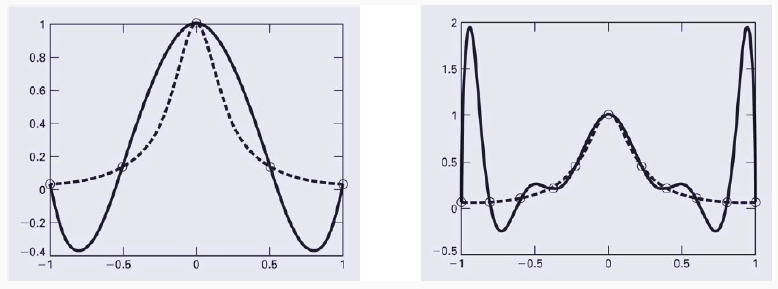
\includegraphics[width=0.5\linewidth]{fig/kurven_interpolieren}
	\caption{Möglichkeit der Darstellung von Kurven}
	\label{fig:kurven_interpolieren}
\end{figure}
Nehmen wir die naive Variante und versuchen, die Kurve durch ein einfaches Polyom darzustellen, also irgendwas in der Form von:
\begin{displaymath}
f(x) = a_0 + a_1x + a_2x^2 + \dots + a_nx^n
\end{displaymath}
Leider nützt uns diese Variante nicht wirklich. Denn die durchgezogenen Linien zeigen, dass diese nie wirklich an die echte Kurve herankommt - mit mehr definierten Punkten wird es sogar noch schlimmer - siehe der rechte Teil der Grafik. Wir müssen also etwas besseres haben.

\subsubsection{Beispielrechnung - Methode der unbestimmten Koeffizienten}
\begin{figure}[!ht]
	\centering
	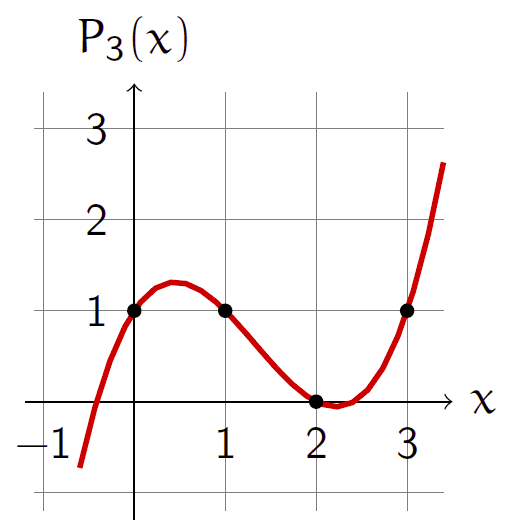
\includegraphics[width=0.3\linewidth]{fig/unbestimmte_koeffizienten}
	\caption{Beispiel Kurve}
	\label{fig:unbestimmte_koeffizienten}
\end{figure}

Wir können also folgende Punkte aus der Kurve lesen: \((0,1)\), \((1,1)\), \((2,0)\), \((3,1)\). Wir können also für die Gleichung

\begin{displaymath}
f(x) = a_0 + a_1x + a_2x^2 + a_3x^3
\end{displaymath}
für den ersten Punkt \(x = 0, y = 1\) wäre die Gleichung also:

\begin{displaymath}
1 = a_0 + a_1\cdot 0 + a_2\cdot 0 + a_3\cdot 0 = a_0
\end{displaymath}

Wir können das auch in einer Matrix darstellen;

\begin{displaymath}
\begin{pmatrix}
	1 & 0 & 0 & 0 \\
	1 & 1 & 1 & 1 \\
	1 & 2 & 4 & 8 \\
	1 & 3 & 9 & 27\\
\end{pmatrix}
\begin{pmatrix}
a_0 \\
a_1 \\
a_2 \\
a_3
\end{pmatrix}
= 
\begin{pmatrix}
1 \\
1 \\
0 \\
1
\end{pmatrix}
\end{displaymath}
und lösen die dann auf mittels Maple oder so - weil von Hand ist ja uncool \& lahm.
Nachteil an dieser Methode ist, dass es eben lahm ist, man muss wenn sich ein Punkt ändert immer das komplette Gleichungssystem wieder lösen. Die Lösung wäre auf jeden Fall:
\begin{displaymath}
f(x) = 1 + \frac{3}{2}x - 2x^2 + \frac{1}{2}x^3
\end{displaymath}
\subsubsection{Beispielrechnung - Methode nach Lagrange}
Wollen wir keine Gleichungssysteme lösen, so lässt uns Lagrange von der Qual erlösen. Schlechter Reim - ist aber trotzdem so.

Nehmen wir wieder wie Kurve aus Abbildung \ref{fig:unbestimmte_koeffizienten}. Wir haben wieder die bekannten Punkte, wobei der erste Punkt dann \(x_0 = 0\) und \(f(x_0) = 1\)  wäre usw.

Wir definieren dann Gleichungen wie in Abbildung \ref{fig:lagrange_gleichungen}.
\begin{figure}[!ht]
	\centering
	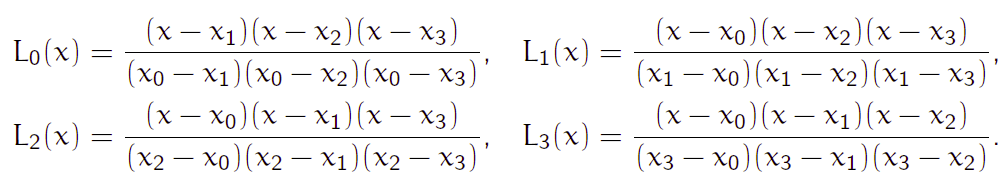
\includegraphics[width=0.7\linewidth]{fig/lagrange_gleichungen}
	\caption{Lagrange Gleichungen}
	\label{fig:lagrange_gleichungen}
\end{figure}
Die Funktion \(L_0(x)\) hat dann die Eigenschaft, dass sie an der Stelle \(x_0 = 1\) ist und an allen anderen Stützstellen, also \(L_0(x_1) = L_0(x_2) = \dots = 0\)  ist. Die Funktion \(L_1(x)\) hat dieselbe Eigenschaft, einfach ist sie an der Stelle \(x_1 = 0\). Dasselbe für die weiteren Gleichungen. Jetzt können wir einfach unsere Gleichung aufstellen:
\begin{displaymath}
f(x) = L_0(x)f(x_0) + L_1(x)f(x_1) + L_2(x)f(x_2)+ L_3(x)f(x_3)
\end{displaymath}
Was dann auch schon die Lösung ist.

Erklärung dazu; Mit den aufgestellten \(L_n\) Gleichungen können wir ja einfach die Stützstellen beliebig 'verschieben' - was wir zum Schluss mit den Faktoren \(f(x_0)\) auch machen. (Anmk. Autor - evt kann das jemand noch besser erklären, ich schreib jetzt einfach mal weiter im Text).
\subsection{Methode nach Newton}
Kommt wahrscheinlich nicht - war ja auch nicht in den Übungen vorhanden.
\section{Approximierende Splines}
Wir definieren einfach irgendwelche Punkte im Raum und bestimmen jeweils die Funktion zwischen den Punkten - diese ist eine Polynomiale Funktion max. 3 Grades. Die Kurve muss dann nicht durch die Punkte gehen.

\begin{figure}[!ht]
	\centering
	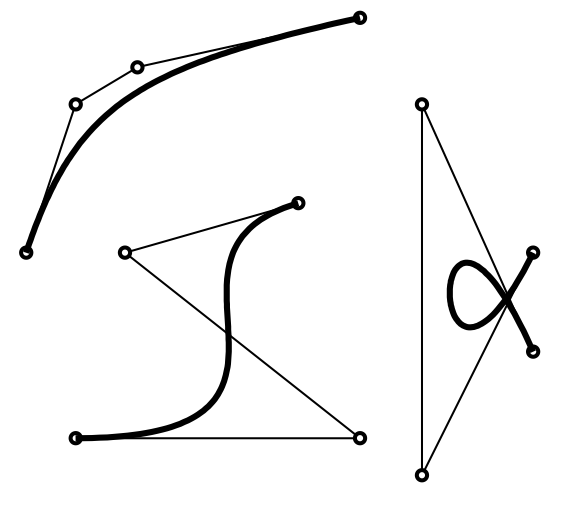
\includegraphics[width=0.3\linewidth]{fig/splines}
	\caption{Splines}
	\label{fig:splines}
\end{figure}

\subsection{Lineare Interpolation - Lineare Bézier Splines}
Wir haben einfach eine Linie mit den Anfangs \(P_0\) und Endpunkten \(P_1\). Jetzt müssen wir diese wahnsinnig schwierig beschreiben. Hier ist immer \(t \leq t \leq 1\).
\begin{enumerate}
	\item \(P(t) = (1-t)P_0+t\cdot P_1\)
	\item \(P(t) = (P_1 - P_0)\cdot t + P_0\)
	\item \(P(t) = (P_1, P_0) \begin{pmatrix}
	-1 & 1 \\1 & 0
	\end{pmatrix}\begin{pmatrix}
	t \\ 1
	\end{pmatrix}\)
\end{enumerate}
\subsection{Quadratische Bézier Splines}
\begin{figure}[!ht]
	\centering
	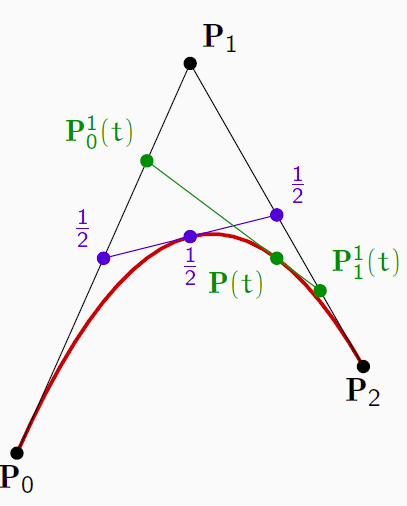
\includegraphics[width=0.2\linewidth]{fig/quadratic_bezier_spline}
	\caption{Quadratische Bézier Splines}
	\label{fig:quadratic_bezier_spline}
\end{figure}
Quadratische Bézier Splines sind eigentlich dasselbe wie die linearen Bézier Splines - einfach wird zwischen den linearen Splines nochmals interpoliert - yo dawg I heard you like interpolieren. In der Abbildung \ref{fig:quadratic_bezier_spline} sieht man das schön. Grafisch kann man das dort auch super erklären - denn vom Punkt in der Mitte zwischen \(P_0\) und \(P_1\)  wird einfach eine Linie gezogen zum Punkt in der Mitte zwischen \(P_1\) und \(P_2\) und dann in der Mitte dieser Linie ist dann der mittlere Punkt der fertigen Kurve. Wir rechnen also die 2 linearen Repräsentationen der Linien zusammen und das geht so:

Man hat zwei lineare Bézier Splines, die so definiert sind:
\begin{displaymath}
P^1_0(t) = (1-t)P_0 + t\cdot P_1
\end{displaymath}
\begin{displaymath}
P^1_1(t) = (1-t)P_1 + t\cdot P_2
\end{displaymath}

Jetzt setzt man diese einfach in die normale Bézier Repräsentation ein - also eine Funktion in die Funktion einfügen.
\begin{displaymath}
P(t) = (1-t)P^1_0(t) = t\cdot P^1_1(t)
\end{displaymath}
Dann muss mans nur noch auflösen et voila:
\begin{displaymath}
P(t) = (1-t)^2P_0 + 2(1-t)t\cdot P_1+t^2P_2
\end{displaymath}
Das, meine Kinder, wäre der ganze Zauber. Tschüss \& bis zum nächsten Mal!

\subsection{Kubische Bézier Splines}
Hehe, jetzt dachtest Du schon du bist fertig. Aber es wird nicht schwieriger. Wir haben jetzt einfach 4 Kontrollpunkte (\(P_0, \dots P_3)\))statt 3, also haben wir alle Definitionen:
\begin{displaymath}
P^1_0(t) = (1-t)P_0 + t\cdot P_1
\end{displaymath}
\begin{displaymath}
P^1_1(t) = (1-t)P_1 + t\cdot P_2
\end{displaymath}
\begin{displaymath}
P^1_2(t) = (1-t)P_2 + t\cdot P_3
\end{displaymath}
Jetzt müssen wir alle 4 Gleichungen zusammenfügen:
\begin{displaymath}
P^2_1(t) = (1-t)P^1_0(t) = t\cdot P^1_1(t)
\end{displaymath}
\begin{displaymath}
P^2_2(t) = (1-t)P^1_1(t) = t\cdot P^1_2(t)
\end{displaymath}
Und diese dann nochmals in tha mix schmeissen:
\begin{displaymath}
P(t) = (1-t)P^2_1(t) = t\cdot P^2_2(t)
\end{displaymath}
Was dann wieder aufgelöst:
\begin{displaymath}
P(t) = (1-t)^3P_0+3(1-t)^2\cdot t\cdot P_1+3(1-t)t^2P_2+t^3P_3
\end{displaymath}
ergibt. Dem aufmerksamen Leser wird nicht entgangen sein, dass diese Bézier Splines Eigenschaften vom Pascal'schen Dreieck haben.

\subsection{Bernsteinpolynome}
Nicht aufgeben! Kurz ein Schluck Wasser und weiter gehts. Es ist jetzt einfach das Ganze Bézier Splies Zeugs - einfach nochmals verallgemeinert. Wir vorhin angetönt - dem aufmerksamen Leser wird ja nicht entgangen sein, dass die Formel der Bézier Kurve irgendwie so ein Muster ähnlich dem Pascal'schen Dreieck hat.
\begin{figure}[!ht]
	\centering
	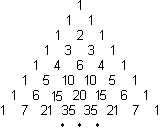
\includegraphics[width=0.2\linewidth]{fig/pascalsches_dreieck}
	\caption{Pascal'sches Dreieck}
	\label{fig:pascalsches_dreieck}
\end{figure}
Die Bausteine von Bézier Splines sind ja auch immer dieselben - also irgendwas mit \((1-t)\) und \(t\) selbst kommt auch irgendwie immer vor. Nehmen wir nochmals das Beispiel vom Kubischen Bézier Spline und zerlegen die End-Formel in die Summanden und nehmen noch kurz die Punkte nochmals raus:

\begin{displaymath}
1\cdot (1-t)^3
\end{displaymath}
\begin{displaymath}
3\cdot (1-t)^2\cdot t
\end{displaymath}
\begin{displaymath}
3\cdot (1-t)\cdot t^2
\end{displaymath}
\begin{displaymath}
1\cdot t^3
\end{displaymath}
Die Faktoren zu Beginn des Terms stellen genau die Binomialkoeffizienten dar. Hier nochmals die Binomiailkoeffizienten-Berechnung:
\begin{displaymath}
\begin{pmatrix}
n \\ i
\end{pmatrix}
= \frac{n!}{i!(n-i)!}
\end{displaymath}
Ersetzen wir die Faktoren doch gleich einmal:

\begin{displaymath}
\begin{pmatrix}
3 \\ 0
\end{pmatrix}\cdot (1-t)^3
\end{displaymath}
\begin{displaymath}
\begin{pmatrix}
3 \\ 1
\end{pmatrix}\cdot (1-t)^2\cdot t
\end{displaymath}
\begin{displaymath}
\begin{pmatrix}
3 \\ 2
\end{pmatrix}\cdot (1-t)\cdot t^2
\end{displaymath}
\begin{displaymath}
\begin{pmatrix}
3 \\ 3
\end{pmatrix}\cdot t^3
\end{displaymath}
Das wärs auch schon gewesen. Denn jetzt können wir daraus die Formel für die einzelnen Teile sagen:
\begin{displaymath}
B^3_i(t)=\begin{pmatrix}3 \\ i\end{pmatrix}(1-t)^{3-i}t^i
\end{displaymath}
Und das sind dann schon die Bernsteinpolynome.
Für \(i\) setzte man dann einfach eine Zahl zwischen 0 und 3 und man erhält dann den Term an der entsprechenden Position.\\ \newline
Jetzt haben wir aber doch am Anfang die Punkte herausgenommen - wir wollen diese jetzt natürlich wieder hineinnehmen. Dazu müssen wir sie nur eben mit dem entsprechenden Term wieder multiplizieren. Die ganze Kubische Bézier Kurve lässt sich dann so schreiben:
\begin{displaymath}
P(t) = \displaystyle\sum_{i=0}^{3} B^3_i(t)\cdot P_i
\end{displaymath}
Jetzt gehen wir ja nur bis 3 - können wir auch bis n gehen? Klar - das sind dann gerade die Bézier Kurven n. Ordnung.
\begin{displaymath}
P(t) = \displaystyle\sum_{i=0}^{n} B^n_i(t)\cdot P_i
\end{displaymath}
Wobei dann die Bernsteinpolynome, also der Teil mit dem \(B\), so definiert sind:
\begin{displaymath}
B^n_i(t)=\begin{pmatrix}n \\ i\end{pmatrix}(1-t)^{n-i}t^i
\end{displaymath}
\subsubsection{Eigenschaften von Bézier Kurven}
\begin{enumerate}
	\item Die Bézier Kurve liegt immer innerhalb der konvexen Hülle des Linienzuges
	\item Die Anzahl der Kontrollpunkte \(P_0, \dots P_n\) bestimmt den Grad \(n\) der Bézier Kurve.
	\item Die Änderung eines Kontrollpunktes bewirkt eine Änderung der gesamten Kurve.
	\item Indem man die stetigen Funktionswerte und Ableitungen voraussetzt, lassen sich Bézier Kurven höheren Grades durch Bézier Kurven niedrigeren Grades zusammensetzen.
\end{enumerate}
Wahnsinnige Mathematische Wortspiele - man kanns auch einfach sagen. Zum ersten Punkt lässt sich sagen, dass in einem konvexen Gebiet jeder Punkt von jedem direkt erreichbar ist, ohne das Gebiet verlassen zu müssen. Also man stelle sich eine Insel im Meer vor. Diese ist konvex, wenn man von jedem x-beliebigen Punkt \textit{trockenen Fusses} an jeden anderen x-beliebigen Punkt kommt. Und die konvexe Hülle beschreibt dann einfach das kleinste Gebiet, welches konvex ist und alle Kontrollpunkte enthält. Abbildung \ref{fig:konvexe_huelle} zeigt in Grau diese konvexe Hülle.
\begin{figure}[!ht]
	\centering
	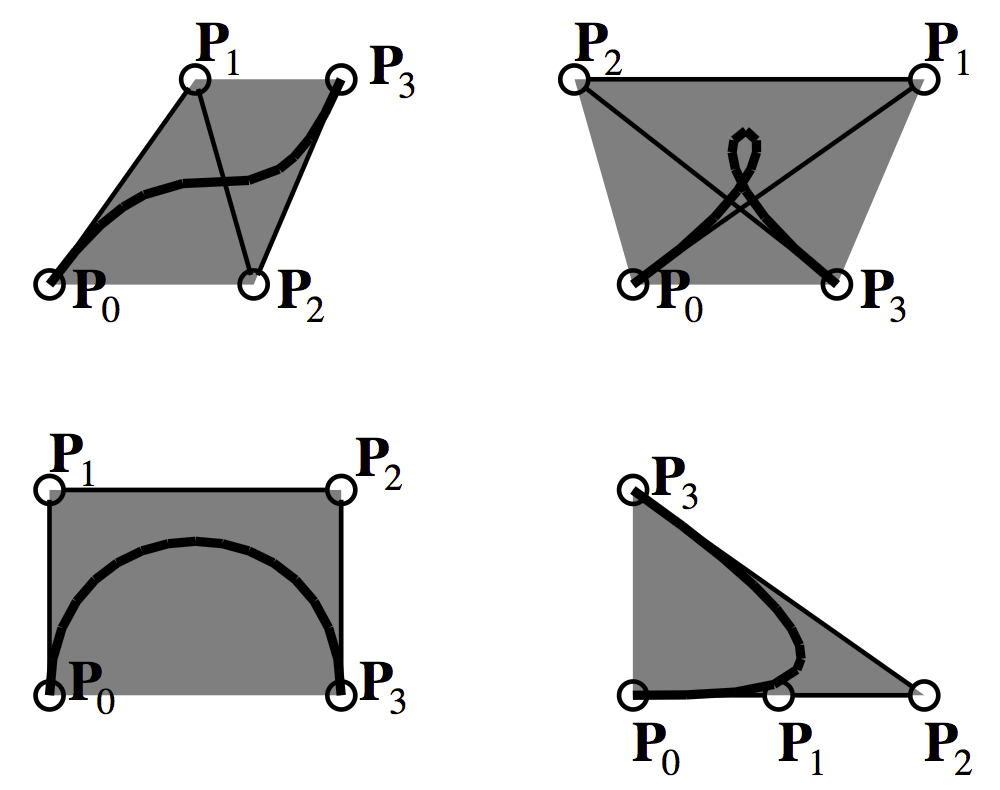
\includegraphics[width=0.3\linewidth]{fig/konvexe_huelle}
	\caption{Konvexe Hülle}
	\label{fig:konvexe_huelle}
\end{figure}
\\ \newline
Die Zusammensetzung von Bézier Kurven setzt ja voraus, dass diese stetig sind. Wir haben folgende Eigenschaften, dass es stetig ist:
\begin{enumerate}
	\item Die Segmente haben an den Endpunkten keine Sprünge / Lücken
	\item Die Segmente haben an den Endpunkten dieselbe erste Ableitung - also nicht eine Kurve in Form von: \(\land\).
	\item Die Segmente haben an den Endpunkten dieselbe zweite Ableitung. Also nicht z.B. eine gerade Linie und gleich anschliessend ein Halbkreis. Das wäre, wie man geradeaus Autofährt und dann direkt eine 180 Grad Kurve kommt und man in unendlich kurzer Zeit das Steuerrad nach rechts drehen sollte, damit man die Kurve 'perfekt' fährt. Also nicht so eine Kurve wie in Abbildung \ref{fig:c2_stetigkeit}.
\end{enumerate}
\begin{figure}[!ht]
	\centering
	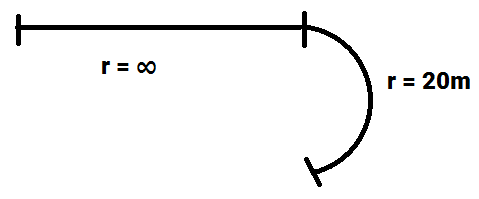
\includegraphics[width=0.2\linewidth]{fig/c2_stetigkeit}
	\caption{Zweite Ableitung ist hier nicht gleich}
	\label{fig:c2_stetigkeit}
\end{figure}
\subsubsection{Zeichnen von Bézier Kurven}
Am besten stellt man 2 Gleichungen auf, eine, die von der \(t\)-Variable abhängig ist und die X-Position ergibt, und die andere welche die Y-Position ergibt. Dann kann man in jedem Taschenrechner für Werte von t von 0 bis 1 diese Gleichungen einfach numerisch lösen und die entsprechenden Punkte einzeichnen und verbinden. Zur Kontrolle empfiehlt sich der Besuch auf folgender Website: \url{https://www.desmos.com/calculator/cahqdxeshd}
\subsection{B Splines \& NURBS}
Laut meinen Notizen nicht Teil der MEP.
\section{Lösungen Übungen}
\subsection{Aufgabe 1}
Der Graph auf der linken Seite beschreibt eine unmöglich durch eine Funktion darstellbaren Graphen dar. Deswegen habe ich jetzt einfach die Achsen umgekehrt, damit eine geforderte Funktion überhaupt erstellbar ist. 
\begin{displaymath}
\begin{pmatrix}
1 & 0 & 0 & 0 \\
1 & 2 & 4 & 8 \\
1 & 3 & 9 & 27 \\
1 & 4 & 16 & 64
\end{pmatrix}
\begin{pmatrix}
c_0 \\
c_1 \\
c_2 \\
c_3 
\end{pmatrix}
= 
\begin{pmatrix}
0 \\
2 \\
0 \\
2 
\end{pmatrix}
\end{displaymath}
Mit dem CAS ergibt sich folgende Lösung:
\begin{displaymath}
c_0= 0 , c_1 = \frac{15}{2}, c_2 = -\frac{19}{4}, c_3 = \frac{3}{4}
\end{displaymath}

\subsection{Aufgabe 2}
Man muss einfach folgende Gleichung aufstellen:
\begin{displaymath}
P\left( t\right) = \left( 1-t\right)^3 \cdot \begin{pmatrix}0 \\ 0\end{pmatrix} + 3\left( 1-t\right)^2\cdot t \begin{pmatrix}2 \\ -4\end{pmatrix} + 3\left( 1-t\right)t^2\begin{pmatrix}5 \\ 6\end{pmatrix} + t^3\begin{pmatrix}9 \\ 0\end{pmatrix}
\end{displaymath}
Wenn man es noch grafisch darstellen möchte, einfach per Taschenrechner ein paar Werte für \(t\), am besten zwischen 0 und 1, ausrechnen und darstellen. Dann sollte es etwa so aussehen:
\begin{figure}[!ht]
	\centering
	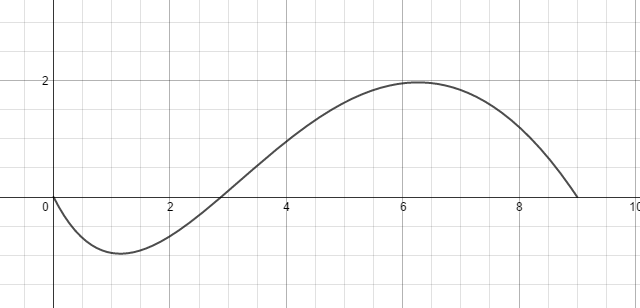
\includegraphics[width=0.5\linewidth]{fig/bezier_aufgabe2}
	\caption{Grafische Lösung Bezier Aufgabe 2}
	\label{fig:bezier_aufgabe2}
\end{figure}

\subsection{Aufgabe 3}
Hier hat man ja durch die normale Bézier Gleichung folgende Gleichung vorgegeben, wobei die mittleren Kontrollpunkte ja unbekannt sind.
\begin{displaymath}
P(t) =  \begin{pmatrix}0 \\ 0\end{pmatrix} (1-t)^3 + 3 \begin{pmatrix}P_x \\ P_y\end{pmatrix}t(1-t)^2+3 \begin{pmatrix}Q_x \\ Q_y\end{pmatrix}t^2(1-t)+ \begin{pmatrix}2 \\ 4\end{pmatrix}t^3
\end{displaymath}
Zusätzlich kann man dann folgende Gleichungen aufstellen, indem man ja diese Constraints setzt:
\begin{displaymath}
P\left(\frac{1}{4}\right) =  \begin{pmatrix}2 \\ 2\end{pmatrix}
\end{displaymath}
\begin{displaymath}
P\left(\frac{3}{4}\right) =  \begin{pmatrix}0 \\ 3\end{pmatrix}
\end{displaymath}
Daraus ergeben sich folgende Gleichungen:
\begin{displaymath}
P_x\left(\frac{1}{4}\right) = 2 = 3 P_x \frac{1}{4}\left(1-\frac{1}{4}\right)^2+3Q_x\frac{1}{4}^2\left(1-\frac{1}{4}\right)+2\frac{1}{4}^3
\end{displaymath}
\begin{displaymath}
P_y\left(\frac{1}{4}\right) = 2 = 3 P_y \frac{1}{4}\left(1-\frac{1}{4}\right)^2+3Q_y\frac{1}{4}^2\left(1-\frac{1}{4}\right)+4\frac{1}{4}^3
\end{displaymath}
\begin{displaymath}
P_x\left(\frac{3}{4}\right) = 0 = 3 P_x \frac{3}{4}\left(1-\frac{3}{4}\right)^2+3Q_x\frac{3}{4}^2\left(1-\frac{3}{4}\right)+2\frac{3}{4}^3
\end{displaymath}
\begin{displaymath}
P_y\left(\frac{3}{4}\right) = 3 = 3 P_y \frac{3}{4}\left(1-\frac{3}{4}\right)^2+3Q_y\frac{3}{4}^2\left(1-\frac{3}{4}\right)+4\frac{3}{4}^3
\end{displaymath}
Das kann man noch vereinfachen, aber so viele Formeln in Latex ist mühsam. Woraus sich mit einem schlauen CAS folgende Lösung ergibt:
\begin{displaymath}
P = \begin{pmatrix}6 \\ 4\end{pmatrix}, Q = \begin{pmatrix}-4 \\ \frac{16}{9}\end{pmatrix}
\end{displaymath}